% RECOMMENDED %%%%%%%%%%%%%%%%%%%%%%%%%%%%%%%%%%%%%%%%%%%%%%%%%%%
\documentclass[graybox]{svmult}
\usepackage[misc]{ifsym}
\usepackage{mathptmx}       % selects Times Roman as basic font
\usepackage{helvet}         % selects Helvetica as sans-serif font
\usepackage{courier}        % selects Courier as typewriter font
\usepackage{type1cm}        % activate if the above 3 fonts are
\usepackage{multirow} 
\usepackage{makeidx}         % allows index generation
\usepackage{graphicx}        % standard LaTeX graphics tool
                             % when including figure files
\usepackage{multicol}        % used for the two-column index
\usepackage[bottom]{footmisc}% places footnotes at page bottom


% see the list of further useful packages
% in the Reference Guide

\makeindex             % used for the subject index
                       % please use the style svind.ist with
                       % your makeindex program


\begin{document}

\title*{Improving Evolutionary Art Audience Interaction by Means of a Kinect Based Non-intrusive Method}
\titlerunning{Analyzing Aud. Percept. of Elitism Opers. by Means of a Kinect B. Non-intr. Method}

\author{Francisco Fern\'andez de Vega   \and Mario Garc\'ia-Valdez \and J.J. Merelo \and Georgina Aguilar \and Cayetano Cruz \and Patricia Hern\'andez}
\authorrunning{Fern\'andez de Vega et al.}

\institute{ F. Fern\'andez de Vega (\Letter) \and  C. Cruz  \at Universidad de Extremadura \\ \email{fcofdez@unex.es} 
\and  M. Garcia-Valdez (\Letter) \and  G. Aguilar \at Instituto Tecnol\'ogico de Tijuana \\ \email{mario@tectijuana.edu.mx}
\and P. Hern\'andez \at University of Seville \\ \email{patriciapahr@gmail.com}
\and J.J. Merelo \at Computer Architecture and Technology, University of Granada, Spain \\ \email{jjmerelo@gmail.com}}

%----------------------------------------------------------------------------------------

% In general, papers should be organized this way. First, general
% framework and problem you want to solve, with the motivation. Second
% the technique you are using to solve it. Finally, conclusions and
% generalization from the problem solution. I would put it this way

% Museum design is an optimization problem that aims to make the
% museum as attractive as possible, at the same time people with
% different interests make the visit comfortably; having a data-based
% approach to organizing exhibitions, producing new works out of
% storage or buying new ones makes it also an interesting
% problem. However, this problem has not been solved numerically so
% far, and there is very little data available to point at
% solutions. An evolutionary art exhibit created by us is an
% interesting testbed, because works of arts are organized in
% "generations", every one of them related to others in the previous
% generation, so inspiration paths are explicit and well known in
% advance. Besides, all works in the exhibition are related. In this
% paper, using this evolutionary art exhibit, we 
% present an off-the shelf system that is able to measure the time
% people spend on every one of the pictures. Analyzing data obtained
% shows that, in general, visitors follow a particular "inspiration"
% track, which, besides indicating that visit time is not random, can
% give a hint to museum designers to create exhibitions clustering
% works that are related to each other by inspiration, rather by
% temporal or other considerations - JJ

\maketitle % Insert title

% This abstract should start with the general problem that is going to
% be solved, then move on to the particular solution that is being
% proposed including the motivation. 
\abstract{This paper analyzes the perception by the audience of
  Evolutionary Works of Art which were produced by means of the
  \textit{unplugged evolutionary algorithm}. % It's not a well-known
                                % thing. Please use an explanation in
                                % the abstract. - JJ
  The long term goal is to study if genetic operations applied by
  artists in an evolutionary art work are consistently understood by
  the audience visiting the art exhibit. % Why do you need to
                                % understand this? What's the
                                % framework that makes this necessary?
  Yet, we need to involve the
  audience in the experiment, so that enough data can be retrieved and
  compared with the way the artists work.
% I don't understand this frase. The long term goal is to study... yet
% we need to involve the audience? We need to involve the audience
% despite our long term goal is to study? Also, you compare what data
% with the way the artists work? - JJ
  Thus, by means of a series of
  experiments that took place in an art exhibit environment, we analyze
  audience behavior using two different approaches, the more
  traditional survey based approach and a new non-intrusive
  methodology which relies on a depth camera. %OK, now you're
                                %talking. You want to research
                                %audience behavior. Is this unique to
                                %the fact that it's genetic art? Or is
                                %it just the way it's happened? Your
                                %objective is to validate one approach
                                %with the other? - JJ
  We show how the latter
  can largely increase the amount of data collected. % which
                                % means... Your problem is "to study
                                % if genetic operators applied... are
                                % consistently understood". Increasing
                                % the amount of data helps towards
                                % that goal? - JJ
   Furthermore, it
  allows to measure both, the time spent by a given person in front of
  an art work, but also to collect additional features about his face,
  where he is looking and basic gesture recognition. These features
  can be used to predict their personal attitude and feelings when
  facing a given art work. Although we describe here preliminary
  results, they allow us to conclude the pertinence of the approach. 
\keywords{Evolutionary Algorithms, Art, Creativity}}

%----------------------------------------------------------------------------------------
%	ARTICLE CONTENTS
%----------------------------------------------------------------------------------------

\section{Introduction}
Evolutionary Algorithms (EAs), as well as its interactive version, the
Interactive EAs (IEA), have been successfully applied to the solution
of optimization problems, as well as to promote creativity when
producing art works \cite{takagi2001interactive}.  Human beings have
played the role of fitness evaluators within the IEA, applying
aesthetic selection when creative processes are faced.  But still new
possibilities for human involvement have been proposed with the
\textit{unplugged evolutionary algorithm}:  it provides new means for
the user to run the algorithm in a different fashion;  main EA
operations are now performed by users, including selection, crossover,
mutation, evaluation, etc, while computers are in charge of more
administrative tasks:  storing and managing populations
\cite{de2014unplugging}. 
  
Since its proposal, UEAs have been successfully applied to generate
collective art works % maybe exhibitions instead of art works. Is
                     % every single artwork collective? In what sense?
                     % - JJ
that have gained public attention:  the latest experiment has produced
a collective art work that has been selected as one of the winners at
the international \textit{Show Your World 2017} art competition
\footnote{http://www.reartiste.com/juried-exhibition-show-your-world-2017/}.
But before that, other art works produced by means of the UEA were
successfully shown to the public in different cities around the world:
Cancún, Amsterdam, Madrid, Vancouver, etc, being one of them awarded
with the ACM Gecco evolutionary art design and creativity award in
2013 \cite{loiacono2014gecco}. 

% You start to mention "the algorithm" here and "the loop" without
% doing any mention of it before. It should be explained, as well as
% the motivation for including the audience in that loop - JJ
Results obtained encouraged us to continue analyzing other components
of the algorithm, but we also understood that not only artists but
also the audience should be included in the loop, to check whether the
evolutionary approach and operations artists apply are coherently
interpreted by the audience.  Although an initial experiment was
% That's what every work of art aims for, being interpreted coherently
% - not. Why is this a motivation? - JJ
performed involving the audience, using a series of questions to be
answered, we quickly understood, as described below, that new
non-intrusive approaches would be needed to properly evaluate audience
experience without disturbing their participation on art exhibits \cite{chou2007museum}.
Actually, previously applied surveys typically produced fatigue in the
audience, when a large number of questions must be answered by
carefully examining the art works shown.  New alternatives are
required that allows to obtain information from the audience, avoiding
fatigue and allowing them to more effectively enjoy the experience. 

This paper presents a proposal for attaining such a goal:  being able
to extract information from the audience while they are simply looking
at the artworks in the exhibit.  By using off-the-shelf human-computer
interaction devices we are able to extract useful information. % about what?
Not
only that, the first experiments show how a correlation may be found
between the data extracted from the audience and some of the genetic
operations applied by artists.  The methodology thus provides a better
% The artists are inspired by previous works, yours and others. This
% inspiration is also present in any other artists. Is the objective
% of the paper to show that people are interested in works of arts
% that are inspired by each other, disregarding others? We should aim
% for a very general problem - JJ
understanding of audience perception, and relevant information that
may allow in the future to improve the UEA.  In addition, the data
extracted allows a first comparison between audience perception and
artists' operations, which is helpful for improving the understanding
of creativity. 

The rest of the paper is organized as follows: Section \ref{loop} presents the literature review. Section \ref{interaction} proposes the methodology aimed at analyzing public reaction. Section \ref{experiments} describes the experiments performed while section \ref{results} presents results.  Finally, we draw our conclusions in Section 5. % Cambiar después por ref


\section{Humans in the EA loop}
\label{loop}
Several decades ago, researchers noticed the interest of allowing
users to interact with the EA, so that some part of the algorithms
were run by users.  This way, the IEA was successfully applied to
problems requiring aesthetic evaluations.  Moreover, new means to
allow users acquire different roles within the EA were envisioned over
the years, thus producing new versions of the EA particularly adapted
to analyze creative processes developed by artists, and the Unplugged
Evolutionary Algorithm (UEA) was born \cite{de2013unplugging}. 

The UEA is a version of the IEA that is ``run'' by artists when
producing a collective art work.  Instead of using the computer to run
the EA and allow users -artists- to interact, computers are removed,
and the human beings are thus in charge of applying every step of the
algorithm, not just evaluation, to produce results:  evaluation,
selection and crossover.  Somehow, the UEA provide artists with a
methodology for artistic creation, while computer scientists gain
access to human creativity analyzed from the point of view of EAs.
% How is this methodology different from the usual one? Artists are
% inspired by other artists and artworks all the time - JJ

The basic idea behind UEAs is to allow artists to apply the EA as the methodology along the art creation process.  Therefore, all operations, including evaluation, selection, crossover, mutation, etc, are performed by human beings, artists, that simultaneously complete a form describing the reasons behind every decision they take, and operation they apply. Thus, once the experiment has been completed, we have a bunch of information to be analyzed and contextualized under the EA perspective, that could help to better understand artists creativity.

Yet, in every artistic process, artists are not the only ones involved.  The work is always produced to be confronted with the public, and thus the audience response is very important for the artists behind the work. Therefore in any computer mediated art process, the reaction of the audience should be studied as carefully as the algorithm is designed.  Thus, we could summarize the main steps of the methodology provided by UEAs as follows:    (i) Unplugging the EA to be executed by artists; (ii) artists produce a collective work while applying the algorithm;  (iii) operations are then analyzed, and the creative process evaluated;  (iv) Audience perception is analyzed and compared with data collected from the previous analysis.

Although in previous works we conducted a number of surveys to check whether the audience properly understood what the artists did \cite{moreno2016analysing}, fatigue of the audience was seen as a drawback of the method.  Actually, the problem of fatigue had already been studied in the context of IEA \cite{frade2010evolution}.  In both cases, a long interaction with the medium produce boredom:  in the IEA the need for the user to evaluate a large number of \textit{individuals} for many generations;  in the UEA when all of the works collectively produced by the artists team -\textit{individuals}- must be analyzed by the audience to answer a series of questions about the genetic operations for every work produced and also figure out the genealogy of the whole work.  Given that 50 or 60 works were produced in previous experiments \cite{de2013unplugging}, \cite{de2014unplugging} a complete series of questions would include five to ten per work, which produce more than 500 questions.  We had instead to focus in just some of the works, thus avoiding to repeat every question 50 or 60 times.  Thus the surveys include about thirty questions.  Even in this case, the audience felt tired and bored, given that for every question a detailed analysis of the picture was required.  Unfortunately, when all of the surveys are completely filled, which is the best situation, partial information is only retrieved, given that many questions had to be removed from the ideal survey for practical reasons, as described above.

Therefore, an alternative is required if we want to capture as much information as possible from the audience, and simultaneously want them to enjoy the experience of visiting an art exhibit:  a different approach must be applied, so that information from the audience can be extracted without disturbing the \textit{art experience}. 

%Therefore, an alternative is required to analyse by means of any kind of sensors audience perception.
We can find in the literature interactive installations where sensors has been already used \cite{tieben2014playful}.  For instance, sensor based interactive installations were set up as a learning auxiliary tool for children with autism \cite{boutsika2014kinect}; similarly, remote operation of machinery and drone robot controls have been implemented using the same kind of sensors \cite{berra2013interfaz}. Examples can be also found in medical applications, such as those related to rehabilitation of patients of Parkinson's disease \cite{pompeu2015effect},  sport related injuries \cite{berra2013interfaz} and burn rehabilitation \cite{parry2014keeping}, all of them using sensors to analyse patients behavior.  We can thus conclude that the flexibility of this kind of devices could be also useful for the goal we pursue.

We thus propose in the third step of our methodology to use a non-intrusive human computer interaction system, which should be capable of obtaining similar information than that acquired before by means of surveys.  Although this goal may be ambitious, we present below our preliminary work towards that goal, which allows us to be optimistic with the idea.  

%In the following sections, we will show how the experiment was design, the technologies employed and the data we obtained from the audience.

%to confront data obtained from the audience in previous experiments by means of surveys, from those that may be directly grab with non-intrusive methods.

%Of particular interest in this work is the elitism operator.  It allows most selected work to survive, so that artists can use it again as a source of inspiration.

%In the experiments described below, six artists were included in the team.  Usually, the experiment begins with artists selecting well known master pieces for the initial population.

\begin{figure}[t]
%\sidecaption
\centering 
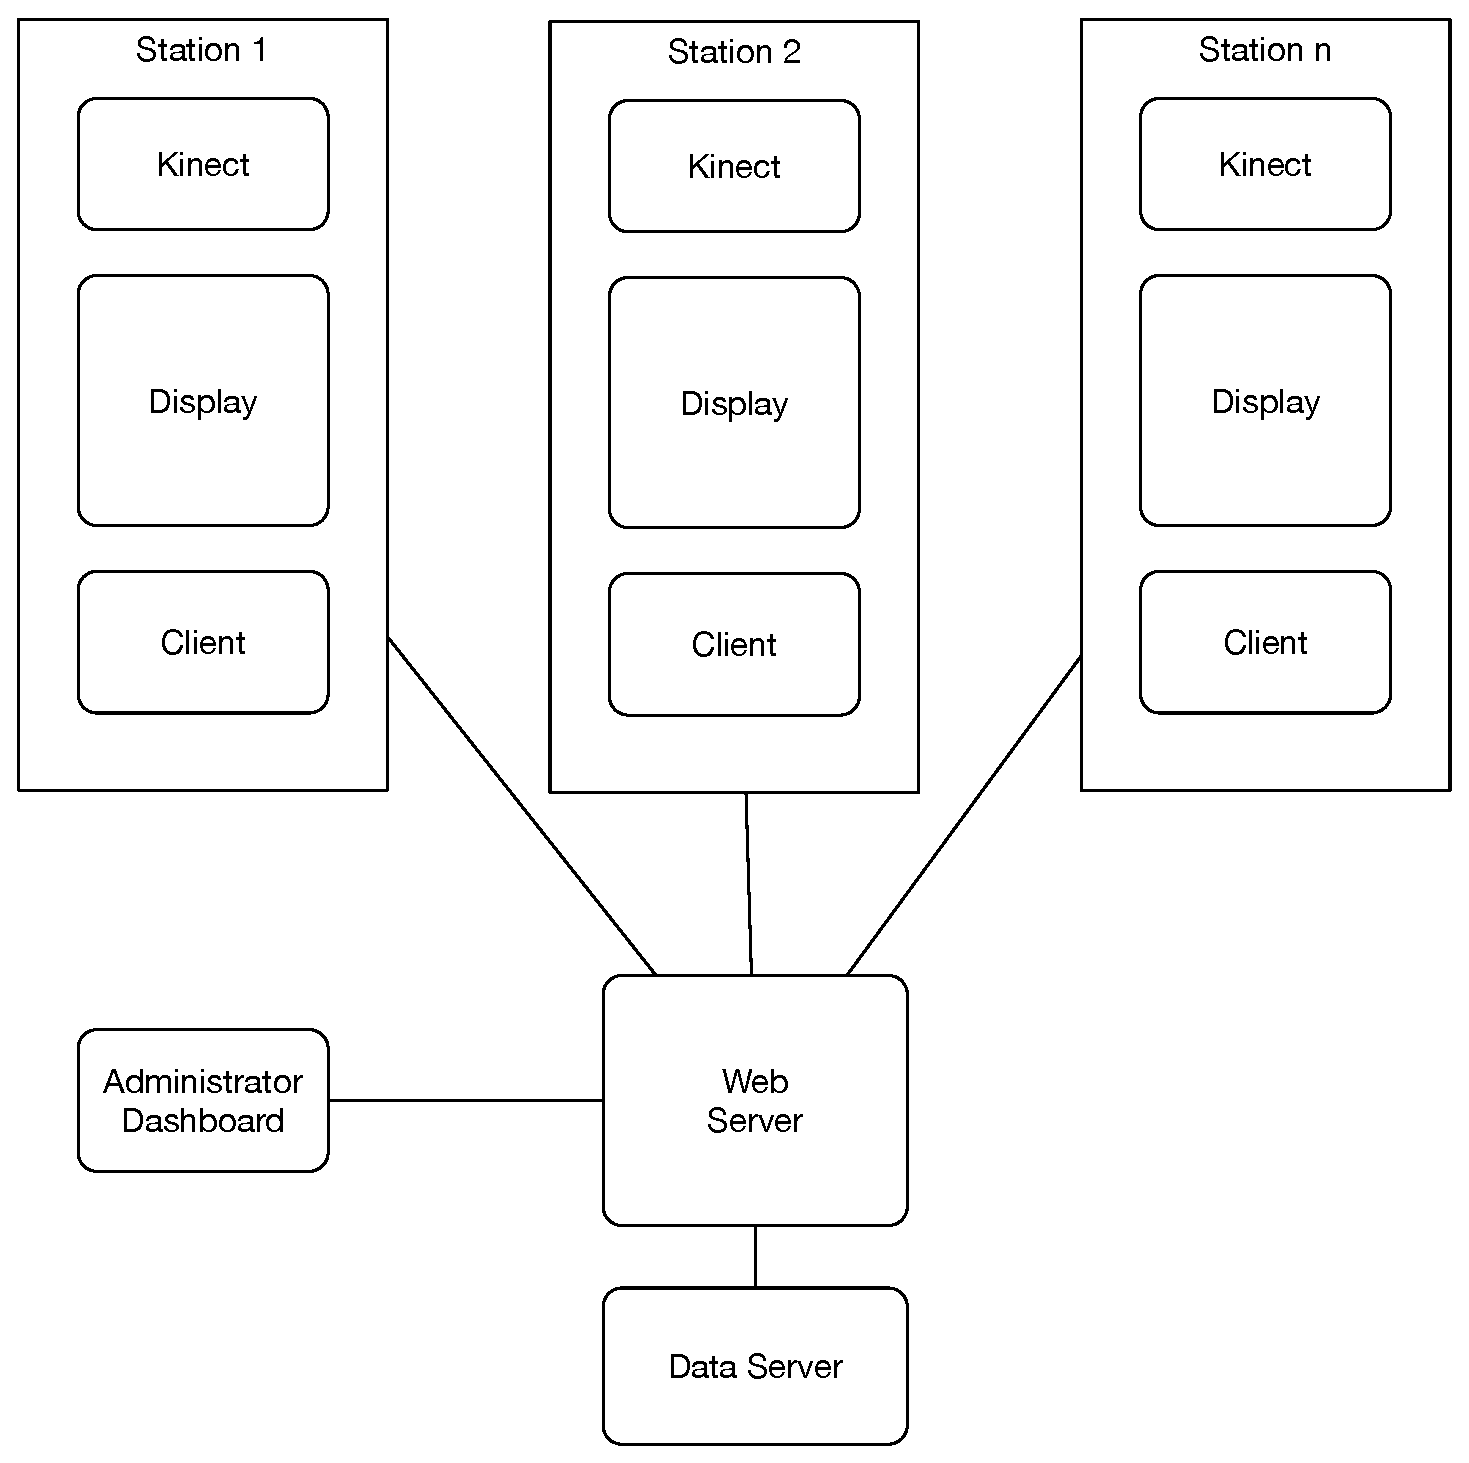
\includegraphics[width=8cm]{img/components.eps}
\caption{ Components of the non-intrusive human-computer interaction system.}
\label{fig:components}       % Give a unique label
\end{figure}

\section{Non-intrusive human-computer interaction system}
\label{interaction}
In order to measure the amount of engagement users have with each painting,
% maybe is not engagement. The amount of response? - Mario  
a natural user interface device is used for facial tracking. In this project in particular the \textit{ Kinect sensor Version 2.0 for Xbox One} was chosen, but other similar sensors could be used; for instance the \textit{RealSense D400} to be available at the beginning of 2018. The Kinect sensor, uses an infrared camera and is capable of measuring depth even in dim light. The software developer kit offers libraries for face and whole body tracking but a disadvantage of the solution is that it has proprietary software. At the time of writing the unit has been discontinued and is no longer been manufactured\cite{kinectOut}. Yet, other alternatives are available from different manufacturers, so that the experiments described below could be reproduced using a different sensor.

The sensor we use can track up to 6 persons at once, and for each face it provides a basic set of information: where the face is, where it is looking, basic expressive information (if the person is smiling), if the face has glasses, and if the eyes are open.  With this information the total amount of interaction can be measured and correlated with engagement. User engagement in this case is defined as the amount of time users spend staring at a painting. This is a simplification, because user engagement in general is a deeper behavior, that occurs when a person is fully concentrated or absorbed in the action that he or she is doing. 

%ESTO LO LLEVO AL FINAL DE LA SECCION PREVIA
%The sensor has been used in several interactive installations  \cite{tieben2014playful}, as a learning auxiliary tool for children with autism \cite{boutsika2014kinect}, remote operation of machinery and drone robot control \cite{berra2013interfaz}. In medical applications has been used in the rehabilitation of patients of Parkinson's disease \cite{pompeu2015effect},  sport related injuries \cite{berra2013interfaz} and burn rehabilitation \cite{parry2014keeping}.

The hardware components of the installation are presented in Fig.~\ref{fig:components}. For each painting or display presenting a group of images there is a sensor station installed.  Each station consists of a compact computer, needed to run the Kinect application, and a Kinect sensor on the top or bottom of the display. For displaying the art a monitor or LCD projector appropriate to the size of the venue or a physical canvas is installed together with the station. Another computer is needed to act as the server, collecting information from all the stations and serving the image files to be presented in each station. A detailed description of each component is presented next.

\begin{figure}[b]
%\sidecaption
\centering 
\includegraphics[width=10cm]{img/face.pdf}

\caption{ Event Frame data, showing face boxes and expressive information for three subjects. Not that in the image captured by the web camera, the positions of the subjects is inverted.}
\label{fig:face}       % Give a unique label
\end{figure}

\subsection{Kinect Client Application}
\label{kinect}
When installing a station, the Kinect application has to be configured simply by setting the Kinect manufacture identifier and the server IP. The Kinect ID will identify all readings sent from the current station, this is important because there could be many sensors reading and sending at the same time. The sensor was set to work at a frame rate of one second, firing a Frame Event only if a face was recognized in that frame. For each Frame Event there could be up to six Face Frames. For each Face Frame the client application sends a \texttt{FrameEvent} object to the server with the following attributes:

\begin{description}
    \item[\texttt{frame\_id}:] This is the frame identifier, several Frame Events could have the same frame\_id because there will be a frame event for each face detected.
    \item[\texttt{kinect\_id}:] As said before, this is the identifier of the station.
    \item[\texttt{date\_time}:] This is a time stamp of the event, this is an important data because it will tie the currently displayed image with the event.
    \item[\texttt{happy}:] This is information is included in the API's \texttt{FreameEvent}, it could have the values: \texttt{yes}, \texttt{no} and \texttt{unknown}.
    \item[engaged:] This attribute indicated if the face is looking at the screen. It has one of the values:\texttt{yes}, \texttt{no} and \texttt{unknown}..

    \item[\texttt{looking\_away}:] Indicates if the user is looking to away from the screen.
    \item[\texttt{face\_index}:] This attribute indicates the index of the Recognized Face is a value from 0 to 5. Once a face is tracked is assigned a value and is kept until losing track. If the same person is out of frame for a few seconds a new face\_id could be generated.
    \item[\texttt{face\_box}:] Screen coordinates of a box drawn for the face. See Figure~\ref{fig:face}.
\end{description}

\begin{figure}[b]
%\sidecaption
\centering 
\includegraphics[width=10cm]{img/dash.pdf}

\caption{ Web-based dashboard application showing readings from a remote station.}
\label{fig:dashboard}       % Give a unique label
\end{figure}

\subsection{Data Server}
Data returned by the stations are stored by the node.js server in a central database, in these experiments both the redis in-memory key-value store and MySQL database system were used. In order to synchronize the reading with the media being displayed at the station, an additional time stamp is added by the server at the time of insertion.

\subsection{Web Client Application} 
In each station, a JavaScript client application is constantly polling the server requesting a file to be displayed. The request includes the Kinect identifier of the station, if there is a new image available the new image is displayed. The Web application, can display images or videos, play audio, or run scripts written in the Processing language.  There is also a dashboard type application for the system administrator. In that application, the current activity of the system is displayed. There is a screen displaying almost in real-time, face-boxes and other Face Frame information from each station. The graphical user interface is presented in Figure~\ref{fig:dashboard}.
%%% Agregado - Mario
On the left side there is an area where the information about the last frames is presented. Each box represents the coordinates of a face as reported by the Kinect sensor, in this case a there are a few overlapped boxes indicating the slight movement of the user. All this information can also be used later to analyze the behavior of users in front of a painting over time. On the right, again the information about the last frames is presented, but indicating the facial expressions.
%%%% 


\subsection{Web Server}
The web server is responsible for coordinating all the stations. A REST API is implemented to deliver media to each station, and also to receive frame events. The server communicates with the back-end databases and file system. Databases contain the Event Frame records and in the file system, images and videos are stored.


\subsection{Post Processing}
Post processing is required to join Frame Event information with the corresponding media presented in the station at the same time. Data is aggregated at different granularities and stored in a MySQL database. With this data, further analysis can be conducted or a fitness estimation could be calculated for each media.     


\section{Experiments}
\label{experiments}
The idea behind the methodology is to confirm that non-intrusive methods for analyzing audience perception can obtain useful information, comparable to those extracted with previous approaches based on surveys, but now avoiding the user fatigue produced by those surveys.

Therefore, we present below a series of experiments aiming at comparing behavior of the audience when surveys are provided, and also when non-intrusive methods are applied.  
%the idea is to conduct a number of experiments that can be compared to results already available for audience perception on the XYZ experiment developed under the UEA methodology \footnote{http://xyz-project.herokuapp.com}.

We will first present a summary of each of the methods, and then will proceed by comparing results obtained with the first one, and published in \cite{moreno2016analysing}, with those that we may obtain using the second one. 

\subsection{Analyzing audience perception by means of surveys}

As already described, a systematic analysis of the audience comments on the results shown are very useful to see if creative processes developed by artists are properly understood by the viewer.  Thus, the first approach for such an analysis was based on surveys conducted among the audience.

We planned a number of art exhibits, and surveys were designed to be collected with useful information for analyzing audience perception.  %Unfortunately, as we will show below in the Results section, surveys had to be elaborated again and even in this case the success was not properly attained.  
Two cities from Spain (Merida and Jerez de la Frontera) an another one from Argentina (Palermo) were selected for the experiments.


\subsection{Capturing data from audience by means of non-intrusive methods}
Alternatively, a different setting was designed to test the non-intrusive methodology described before.
%% 1.- Confirmar como se mostraron los pares de imágenes (cuáles en cada par). 
%% BEGIN Nuevo - Mario
As an experiment, four paintings were exposed in pairs, each pair for one day. Two stations were deployed on the campus of the Tijuana Institute of Technology, in a busy hallway next to the cafeteria, displaying one painting each. The number of students on each day was similar as there was no special event or activity that could increase traffic. Two days before the first experiment a dummy experiment was conducted in order to eliminate the extra attention generated by the new stations in the hallway.
%% END  Nuevo - Mario
On each station a high resolution web camera was also installed, to record the interaction for validation purposes. The four paintings (two pairs) selected for the experiments are: The Kiss by Gustav Klimt (1908) Fig.~\ref{fig:kiss} and Ophelia by John Everett Millais (1852) Fig.~\ref{fig:ophelia} for the first pair to be shown, and The Birth of Venus by Sandro Botticelli (1486) Fig.~\ref{fig:venus} and Impossible Love by Marc Brunet (2006-2016) Fig.~\ref{fig:impossible} as the second pair.

\begin{figure}[t]
\centering 
\includegraphics[width=6cm]{img/klimt-der-kuss-1908.jpg}
\caption{ The Kiss by Gustav Klimt (1908)}
\label{fig:kiss}       % Give a unique label
\end{figure}

\begin{figure}[t]
\centering 
\includegraphics[width=8cm]{img/Ophelia.jpg}
\caption{ Ophelia by John Everett Millais (1852)}
\label{fig:ophelia}       % Give a unique label
\end{figure}

\begin{figure}[t]
\centering 
\includegraphics[width=8cm]{img/Venus.jpg}
\caption{ The Birth of Venus by Sandro Botticelli (1486)}
\label{fig:venus}       % Give a unique label
\end{figure}

\begin{figure}[t]
\centering 
\includegraphics[width=8cm]{img/amorimposible.jpg}
\caption{ Impossible Love by Marc Brunet ()}
\label{fig:impossible}       % Give a unique label
\end{figure}
%VER CUALES DE LOS ANTERIORES ELEMENTOS PUEDEN COMPARARSE CON LOS DATOS DE LA KINECT.

The idea is the to analyze the interaction of users for each of the pairs shown.

\section{Results}
\label{results}
This section presents and compare results obtained with both methods previously described:  (i) survey based approaches;  (ii) non-intrusive methods for audience analysis.

\subsection{Analyzing audience perception by means of surveys}

As described above, three art exhibits were organized with collective works XY and XYZ, and  50 surveys were finally collected, which included questions about relationships among parents-children, elitism, figurativeness, feelings translated (love, fragility, mystery, etc), initial population, etc.  Although surveys allow to ask anything required, the process of collecting surveys, as we show below, was not easy:  more than one thousand people visited the art exhibits but only 50 surveys were correctly filled.

The first art exhibit where surveys were distributed among the audience took place in Jerez de la Frontera, a mid-size southern spanish city. Art students attended the exhibition and were asked to collaborate (see figure \ref{fig:survey}).  Unfortunately, as described in \cite{moreno2016analysing} "The result of the analysis could not be performed
because there were incomplete surveys. The reason was that
students didn't understood properly some of the questions
posed. Another reason is the fatigue due to the number of
questions included".  Thus, this first failed attempt to use surveys as the main source of information led us to re-elaborate the surveys again, and a new questionnaire was formulated,
with smaller number of questions more clearly specified.

\begin{figure}[t]
\centering 
\includegraphics[width=10cm]{img/survey.jpg}
\caption{Students completing the XY survey}
\label{fig:survey}       % Give a unique label
\end{figure}

Therefore, a second attempt to collect information from the audience took place in Palermo, Argentina, during the 10th
Ibero-American Design Meeting 2015, at the University of
Palermo. All viewers were professional designers.  Yet, few people from the audience completed the survey (just 8 surveys completed). Again, the problem was that the audience typically attended an art exhibit to enjoy, and usually refuse surveys because they disturb the otherwise rewarding experience.

Finally, we also showed the work to Industrial Design
Engineering and Product Development students, at the
University of Extremadura, Spain (42 surveys).  They were our own students, and this was the reason for the success:  completing the survey was a compulsory assignment for the subject.  Therefore, only when completing the survey was a compulsory activity for a subject we were able to collect enough information.

Although interesting information was obtained, which finally allowed an analysis of some of the operations applied by artists (see \cite{moreno2016analysing}), our main goal was not achieved, as summarized in table \ref{tab:surveys}.  The main conclusion is that audience refuse to complete surveys when attending art exhibits, so a different mechanism is required to collect useful information for analyzing public's reaction to the artwork on display.

\begin{table}[ht]

\centering
\begin{tabular*}{0.80\textwidth}{@{\extracolsep{\fill}} |l|l|l|l| }
\hline
Type & City & Surveys collected & Audience \\ \hline
Elective   & Jerez (Spain) & 0 & hundreds \\ \hline
Elective & Palermo (Argentina) & 8  & hundreds\\ \hline
Mandatory & Merida (Spain) & 42 & 42 \\ \hline
\end{tabular*}
\caption{Surveys collected.} 
\label{tab:surveys}
\end{table} 


%We describe below how the new non-intrusive methodology, allowed to collect information, without disturbing the exhibit experience.

%As described in \cite{} surveys were conducted among the audience attending art exhibits organized in Cancun, Vancouver, Buenos Aires and Merida.  Yet, the first surveys were discarded:  the number of questions and time required to answer them, were so large that hardly ever the survey was completed.  The fatigue experienced by the users prevented them from completing the surveys.

%Although the experience allowed to improve the surveys, and we were thus able to collect 50 completed ones in the latest art exhibits, the fatigue problem has always been present, and has been the main reason for the attempt described below.

%In any case, the surveys allowed us to confirm some issues \cite{}:

%\begin{itemize}
%\item{Elitism is properly understood:  Usually most selected work from a given generation is the same for artists and audience}
%\item{Both audience and artists prefer figurativism}
%\end{itemize}
 
  Although we have obtained further information regarding how feelings are understood, or mechanism for building the initial generation, we will focus on those shown above for the experiments involving survey-free non-intrusive methods.

\begin{table}[ht]
\centering
\begin{tabular*}{0.80\textwidth}{@{\extracolsep{\fill}} |l|l|r|r|r|r|r| }
\hline
Painting & Expression & yes & no & maybe & unknown & total \\ \hline
\multirow{2}{*}{The Kiss} & happy   & 107 & 266 & 188 & 211 & \multirow{2}{*}{772} \\
                          & engaged & 183 & 466 & 123 & 0   & \\ \hline
\multirow{2}{*}{Ophelia} & happy & 179 & 488 & 294 & 348 & \multirow{2}{*}{1269} \\
 & engaged & 332 & 681 & 256 & 0 &\\ \hline
\multirow{2}{*}{The Birth of Venus} & happy & 188 & 907 & 313 & 1759  & \multirow{2}{*}{3167} \\
 & engaged & 374 & 2545 & 248 & 0 &\\ \hline
\multirow{2}{*}{Impossible Love} & happy & 337 & 1218 & 446 & 3260 & \multirow{2}{*}{5261} \\
 & engaged & 405 & 4474 & 382 & 0 &\\ \hline
\end{tabular*}
\caption{Readings from each station.} 
\label{tab:readings}
\end{table} 

\subsection{Capturing data from audience by means of non-intrusive methods}
In Table \ref{tab:readings}, the total number of frames captured by each sensor is presented for each painting. As mentioned in section \ref{kinect} only those frames with at least one face recognized by the sensor are recorded at a frame rate of two seconds. Each record has the following attributes: painting, happy, engaged. Both \textit{happy} and \textit{engaged} attributes can have one of the following values: \textit{yes}, \textit{no}, \textit{maybe} or \textit{unknown}.  In the table, the column named \textit{total} has the total number of frames captured for each painting. In each row, a breakdown for each of the expressions is presented. For instance, The Kiss had a total of 772 records or frames with faces in them. If we consider the \textit{happy} attribute, out of those 772 records 107 had \textit{yes}, 266 \textit{no}, 188  \textit{maybe} and 211 \textit{unknown}. Even regardless of the expression, the total number of records indicate persons facing the painting, but not necessarily looking directly at it or smiling. The table is ordered by the total number of records, we can see that the paintings of the first day The Kiss and Ophelia had considerably less attention than those of the second day. Again, the traffic on the hallway was the same on both days and they where presented the same amount of time. More people stared at The Impossible Love painting with 5261 records but only a small number of people stared directly at it.  Summarizing, even when the exhibit was located in an open area and the audience was not directly interested in visiting an art exhibit, the methodology has shown how a larger amount of data can be captured.

Yet, we were not only interested in the amount of data, but also in whether data obtained could be trusted.  Therefore an additional survey based experiment was designed so that we can establish a correlation between data obtained by means of surveys and those extracted by sensors.

Therefore, a \textit{Likert} survey was designed and answered by 102 students in an additional experiment at the same university. A small gallery with the previous paintings was presented to students, after receiving a brief introduction to genetic algorithms they were asked to assign fitness values to each painting according to their tastes. The five options where: Like very much, Like, Neutral, Dislike, Dislike very much. These answers can be seen also as a five star rating system, from one to five stars. The result of the survey is shown in Table \ref{tab:survey}.

\begin{table}[ht]
\centering
\begin{tabular*}{\textwidth}{@{\extracolsep{\fill}} |l|l|r|r|r|r|r| }
\hline
Painting & NA & like much & like  & Neutral & Dislike  &  Dislike much \\ \hline
The Kiss & 0 & 18 & 41  & 29 & 14  & 0 \\ \hline
Ophelia  & 1 & 23 & 47  & 19 & 11  & 1 \\ \hline
The Birth of Venus & 0 & 32 & 41  & 24 & 5  & 0 \\ \hline
Impossible Love & 0 & 55 & 23  & 17 & 4  & 3 \\ \hline

\end{tabular*}
\caption{Survey results.} 
\label{tab:survey}
\end{table} 

As we may notice, Ophelia was preferred from the first pair of paintings over the Kiss, while Impossible love was the preferred one from the second pair of paintings.  We can compare these results with those shown in table \ref{tab:readings}:  Ophelia and Impossible love were both the works displaying higher values of happiness and engagement for each of the pairs shown.

But we can also compare this results with artists preferences when developing the evolutionary art work, which allows us to analyse wheather best valued art works are the same for the audience and the artists.  If we check \textit{elitism} information for both experiments XY (Ophelia and Birth of Venus) and XYZ (The Kiss and Impossible Love), we see that Ophelia was second most selected works for XY \cite{arteevolutivo}, while Impossible Love was also second most selected one by artists in XYZ experiment \cite{moreno2016analysing}.  Although there was no exact coincidence in the most valued work of art, in both cases the chosen works were in the group of the most selected.  Thus we can conclude that although not a perfect coincidence in the preferred work, there is a correlation between artist's preferences and audience ones.  To the best of our knowledge, this is the first time such an information is automatically captured from audience when evolutionary art is displayed.

Although still preliminary, we can thus conclude, that the results show that sensor-based non-intrusive methods allows to capture useful information when analyzing audience perception:  the audience is not disturbed, the amount of data increases significantly, and data obtained allows to understand and confront audience perception with artists creativity.  Future and more extensive experiments be useful to confirm the appropriateness of the approach presented.

\section{Conclusions}
%\input{Conclusions}

This paper describes a new non-intrusive approach to the analysis of audience perception when attending art exhibits.

Althouhg survey-based methods were used in previous works to extract useful information from the audience, a detailed analysis of the participation rates described in this paper allows us to see that the audience generally rejects surveys, and simply prefers to enjoy the art exhibits.  A very low paticipation rate (50 over 1000) documented made us consider alternatives.

Thus a new sensor based methodology has been developed that allow us to capture audience perception avoiding public nuisance with polls. 

A couple of experiments has been employed to capture several thousand interaction data, with useful information about the interest, engagement and feelings.  Moreover, data has been confronted with another survey based experiment, and the correlation between sensor based information and answer provided by users is direct. 

Finally, data extracted has been confronted with artists way of working in the evolutionary context, and has provide useful information to see a relationship between elitism operations and audienced preferred works.

We believe that these encouraging results allows us to see the interest of the approach, and will allow to design new art exhibitions that provide a massive capture and analysis of the public's reaction.

\section*{Acknowledgements}
\sloppypar  The authors would like to thank Spanish Ministry of Economy,
Industry and Competitiveness and European Regional
Development Fund (FEDER) under projects TIN2014-56494-
C4-4-P (Ephemec) and TIN2017-85727-C4-4-P (DeepBio);
Junta de Extremadura FEDER, projects GR15068, GRU10029 and IB16035
Regional Government of Extremadura, Consejer\'ia of Economy
and Infrastructure, FEDER.



%----------------------------------------------------------------------------------------
%	REFERENCE LIST
%----------------------------------------------------------------------------------------
\bibliographystyle{spmpsci}
\bibliography{neo}


%----------------------------------------------------------------------------------------

\end{document}

